\documentclass[12pt,a4paper,twoside,UTF8,fontset=none]{ctexart}

\usepackage[
  top=22mm,
  bottom=26mm,
  inner=26mm,
  outer=22mm,
  headheight=25pt,
  headsep=7mm,
  footskip=12mm
]{geometry}
\usepackage{fontspec}
\usepackage{amsmath,amssymb}
\usepackage[table]{xcolor}
\usepackage{array,booktabs,tabularx,longtable}
\usepackage{hhline}
\usepackage{needspace}
\usepackage{tikz}
\usetikzlibrary{calc}
\usepackage{graphicx}
\usepackage{titlesec}
\usepackage{fancyhdr}
\usepackage{hyperref}
\usepackage{enumitem}
\usepackage{microtype}

\defaultfontfeatures{Ligatures=TeX}
\IfFontExistsTF{TeX Gyre Heros}{%
  \setmainfont{TeX Gyre Heros}\setsansfont{TeX Gyre Heros}
}{%
  \IfFontExistsTF{Nimbus Sans}{%
    \setmainfont{NimbusSans-Regular.otf}[BoldFont=NimbusSans-Bold.otf,ItalicFont=NimbusSans-Italic.otf,BoldItalicFont=NimbusSans-BoldItalic.otf]
    \setsansfont{NimbusSans-Regular.otf}[BoldFont=NimbusSans-Bold.otf,ItalicFont=NimbusSans-Italic.otf,BoldItalicFont=NimbusSans-BoldItalic.otf]
  }{\setmainfont{Latin Modern Sans}\setsansfont{Latin Modern Sans}}
}
\setmonofont{Latin Modern Mono}
% 华文行楷：电脑需已安装该字体
\newCJKfontfamily\coverxingkai[
  BoldFont=STXingkai
]{STXingkai}
\newfontfamily\coverenglish{EB Garamond}

\newfontfamily\abstractenglish{TeX Gyre Pagella}%TeX Gyre Pagella，Libertinus Serif，Latin Modern Roman，Palatino，EB Garamond
% Compile with XeLaTeX. Prefer the supplied fonts; otherwise use installed CJK fonts.
\IfFileExists{NotoSansSC-Regular.ttf}{%
  \setCJKmainfont[Path=./,BoldFont=NotoSansSC-Bold.ttf]{NotoSansSC-Regular.ttf}
  \setCJKsansfont[Path=./,BoldFont=NotoSansSC-Bold.ttf]{NotoSansSC-Regular.ttf}
}{%
  \IfFontExistsTF{Noto Sans CJK SC}{%
    \setCJKmainfont{Noto Sans CJK SC}
    \setCJKsansfont{Noto Sans CJK SC}
  }{%
    \setCJKmainfont{FandolHei-Regular}[BoldFont=FandolHei-Bold]
    \setCJKsansfont{FandolHei-Regular}[BoldFont=FandolHei-Bold]
  }
}
% Optional image assets: the document also compiles without them.
\newcommand{\gbulogo}[1]{%
  \IfFileExists{GBU-logo-horizontal-blue.png}{%
    
\includegraphics[width=#1]{GBU-logo-horizontal-blue.png}%
  }{%
    {\color{GBUBlue}\sffamily\coverxingkai\bfseries\LARGE 大湾区大学\par}
    \vspace{1mm}{\color{GBUBlue}\sffamily\coverxingkai\large GREAT BAY UNIVERSITY\par}%
  }
}

\definecolor{GBUBlue}{RGB}{13,0,178}
\colorlet{GBUBlueDark}{GBUBlue!70!black}
\colorlet{GBUBlueLight}{black!3!white}
\colorlet{GBUSessionFill}{black!9!white}
\definecolor{GBUOrange}{RGB}{255,74,5}
\definecolor{GBUPurple}{RGB}{128,0,196}
\definecolor{GBUOchre}{RGB}{164,120,32}
\definecolor{GBUSilver}{RGB}{210,211,207}
\definecolor{GBUBackdrop}{RGB}{245,246,246}
\definecolor{GBUText}{RGB}{0,0,0}
\colorlet{GBURule}{black!45!white}

\hypersetup{
  hidelinks,
  pdfprintscaling=None,
  pdfduplex=DuplexFlipLongEdge,
  pdftitle={第三届大湾区拓扑会议},
  pdfauthor={大湾区大学理学院}
}

\setlength{\parindent}{2em}
\setlength{\parskip}{0.35em}
\setlength{\emergencystretch}{2em}
\setlength{\arrayrulewidth}{0.5pt}
\setcounter{secnumdepth}{0}
\renewcommand{\baselinestretch}{1.16}
\clubpenalty=10000
\widowpenalty=10000
\displaywidowpenalty=10000
\raggedbottom

\titleformat{\section}
  {\color{GBUBlue}\sffamily\coverxingkai\bfseries\Large}
  {}{0pt}{}
  [\vspace{0.25em}{\color{GBUOrange}\titlerule[1.1pt]}]
\titlespacing*{\section}{0pt}{0.8em}{0.9em}

\titleformat{\subsection}
  {\color{GBUBlueDark}\sffamily\coverxingkai\bfseries\large}
  {}{0pt}{}
\titlespacing*{\subsection}{0pt}{1.0em}{0.55em}

% The motto and page number are centred on the physical sheet, including
% even pages with mirrored binding margins. The cover and its blank reverse
% remain unnumbered; conference information starts at body page 1.
\newcommand{\printfooter}{%
  \begin{tikzpicture}[remember picture,overlay]
    \node[anchor=base,inner sep=0pt,text=GBUBlue,
      font=\sffamily\coverxingkai\fontsize{8}{10}\selectfont]
      at ([yshift=20mm]current page.south)
      {基础扎实、视野开阔、知行合一、融会贯通};
    \node[anchor=base,inner sep=0pt,text=GBUText,
      font=\sffamily\coverxingkai\fontsize{9}{11}\selectfont]
      at ([yshift=13mm]current page.south) {\thepage};
  \end{tikzpicture}%
}

\pagestyle{fancy}
\fancyhf{}
\fancyhead[L]{\small\color{GBUBlueDark}\coverxingkai 第三届大湾区拓扑会议}
\fancyhead[R]{\small\color{GBUBlueDark}\coverxingkai 会议手册}
\fancyfoot[C]{\printfooter}
\renewcommand{\headrulewidth}{0.45pt}
\renewcommand{\headrule}{\hbox to\headwidth{\color{GBURule}\leaders\hrule height \headrulewidth\hfill}}
\fancypagestyle{printdivider}{%
  \fancyhf{}
  \fancyfoot[C]{\printfooter}
  \renewcommand{\headrulewidth}{0pt}
  \renewcommand{\headrule}{}
}
\fancypagestyle{plain}{%
  \fancyhf{}
  \fancyfoot[C]{\printfooter}
  \renewcommand{\headrulewidth}{0pt}
  \renewcommand{\headrule}{}
}

\newcolumntype{L}[1]{>{\raggedright\arraybackslash}p{#1}}
\newcolumntype{B}[1]{>{\raggedright\arraybackslash\bfseries\leavevmode\color{GBUBlueDark}}p{#1}}
\newcolumntype{C}[1]{>{\centering\arraybackslash}p{#1}}
\newcolumntype{Y}{>{\raggedright\arraybackslash}X}
% Schedule-only columns: centre text horizontally and vertically.
\newcolumntype{S}{>{\centering\arraybackslash}X}
\newcolumntype{D}[1]{>{\centering\arraybackslash}m{#1}}

\newcommand{\diamondrule}{%
  \begin{center}
    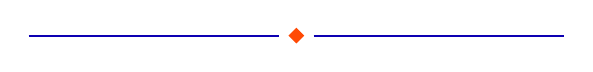
\begin{tikzpicture}
      \draw[GBUBlue, line width=0.7pt] (-3.4,0)--(-0.22,0);
      \fill[GBUOrange] (0,0.10)--(0.10,0)--(0,-0.10)--(-0.10,0)--cycle;
      \draw[GBUBlue, line width=0.7pt] (0.22,0)--(3.4,0);
    \end{tikzpicture}
  \end{center}
}

\newcommand{\sessionrow}[2]{%
  \rowcolor{GBUSessionFill}
  \multicolumn{3}{|c|}{\color{GBUText}\bfseries #1\quad 主持人：#2}\\
  \hhline{|---|}
}

\newcommand{\speakerdisplay}[2]{%
  \textbf{#1}%
  \if\relax\detokenize{#2}\relax
  \else
    \par\vspace{0.04em}{\scriptsize\color{GBUText}#2}%
  \fi
}

\newcommand{\talkrow}[3]{%
  #1 & #2 & #3\\
  \hhline{|---|}
}

\newcommand{\breakrow}[1]{%
  \rowcolor{black!3!white}
  #1 & \multicolumn{2}{c|}{\color{GBUBlueDark}\bfseries 自由交流}\\
  \hhline{|---|}
}

% #1：报告题目
% #2：报告人姓名
% #3：单位
% #4：报告时间
\newenvironment{talkabstract}[4]{%
  \par\addvspace{1.25em}
  \Needspace{13\baselineskip}
  \noindent\begin{minipage}{\textwidth}
  \phantomsection
  \noindent
  \begin{tikzpicture}
    \node[
      anchor=north west,
      text width=\dimexpr\textwidth-0.70cm\relax,
      align=left,
      inner sep=0pt
    ] (talkhead) at (0.45,0) {%
      {\hyphenpenalty=10000\exhyphenpenalty=10000
       \color{GBUBlueDark}\sffamily\coverenglish
       \bfseries\large #1\par}
      \vspace{0.30em}
      {\sffamily\small
 \textbf{报告人：#2（#3）}%
 \hspace{1.5em}%
 时间：\mbox{#4}\par}
    };
    \fill[GBUBlue]
      ([xshift=-0.45cm]talkhead.north west)
      rectangle
      ([xshift=-0.31cm]talkhead.south west);
  \end{tikzpicture}\par\nobreak
  \vspace{0.25em}
  \noindent{\color{GBUOrange}\rule{\textwidth}{1.0pt}}
  \par\nobreak\vspace{0.20em}

  \noindent{%
    \color{GBUBlue}\sffamily\coverxingkai\bfseries
    报告摘要 / \coverenglish Abstract
  }\par

  \abstractenglish
  \fontsize{12}{15.5}\selectfont
}{%
  \par\normalsize
  \par\vspace{0.75em}
  \noindent{\color{GBURule}\rule{\textwidth}{0.45pt}}
  \end{minipage}\par\addvspace{0.2em}
}

\newenvironment{talkabstractt}[3]{%
  \par\addvspace{1.25em}
  \Needspace{13\baselineskip}
  \noindent\begin{minipage}{\textwidth}
  \phantomsection
  \noindent
  \begin{tikzpicture}
    \node[
      anchor=north west,
      text width=\dimexpr\textwidth-0.70cm\relax,
      align=left,
      inner sep=0pt
    ] (talkhead) at (0.45,0) {%
      {\hyphenpenalty=10000\exhyphenpenalty=10000
       \color{GBUBlueDark}\sffamily\coverenglish \bfseries\large #1\par}
      \vspace{0.30em}
      {\sffamily\bfseries 报告人 / Speaker：#2 （#3）\par}  
    };
    \fill[GBUBlue]
      ([xshift=-0.45cm]talkhead.north west)
      rectangle
      ([xshift=-0.31cm]talkhead.south west);
  \end{tikzpicture}\par\nobreak
  \vspace{0.25em}
  \noindent{\color{GBUOrange}\rule{\textwidth}{1.0pt}}
  \par\nobreak\vspace{0.20em}

  \noindent{\color{GBUBlue}\sffamily\coverxingkai\bfseries 报告摘要 / \coverenglish Abstract}\par
  % 摘要正文：Termes，字号11pt，行距15.5pt
  \abstractenglish
  \fontsize{12}{15.5}\selectfont
}{%
  \par\normalsize
  \par\vspace{0.75em}
  \noindent{\color{GBURule}\rule{\textwidth}{0.45pt}}
  \end{minipage}\par\addvspace{0.2em}
}

\newcommand{\bio}[1]{%
  \par\vspace{0.55em}
  \Needspace{10\baselineskip}
  \noindent{\color{GBUBlue}\sffamily\coverxingkai\bfseries 个人简介 / \coverenglish  Biography}\par
  \vspace{0.5em}\small #1\par
}

\begin{document}
\color{GBUText}
\hypersetup{pageanchor=false}

% --------------------------------------------------------------------------
% Cover: image background beneath the existing cover typography.
% --------------------------------------------------------------------------
\newgeometry{top=12mm,bottom=15mm,left=20mm,right=20mm}
\thispagestyle{empty}
\thispdfpagelabel{封面}
\nopagecolor % No solid GBUBlue page background on the front cover.
% Draw once, on the background layer, so cover lettering remains above the image.
\AddToHookNext{shipout/background}{%
  \begin{tikzpicture}[remember picture,overlay]
    \node[anchor=center,inner sep=0pt,outer sep=0pt]
      at (current page.center) {%
        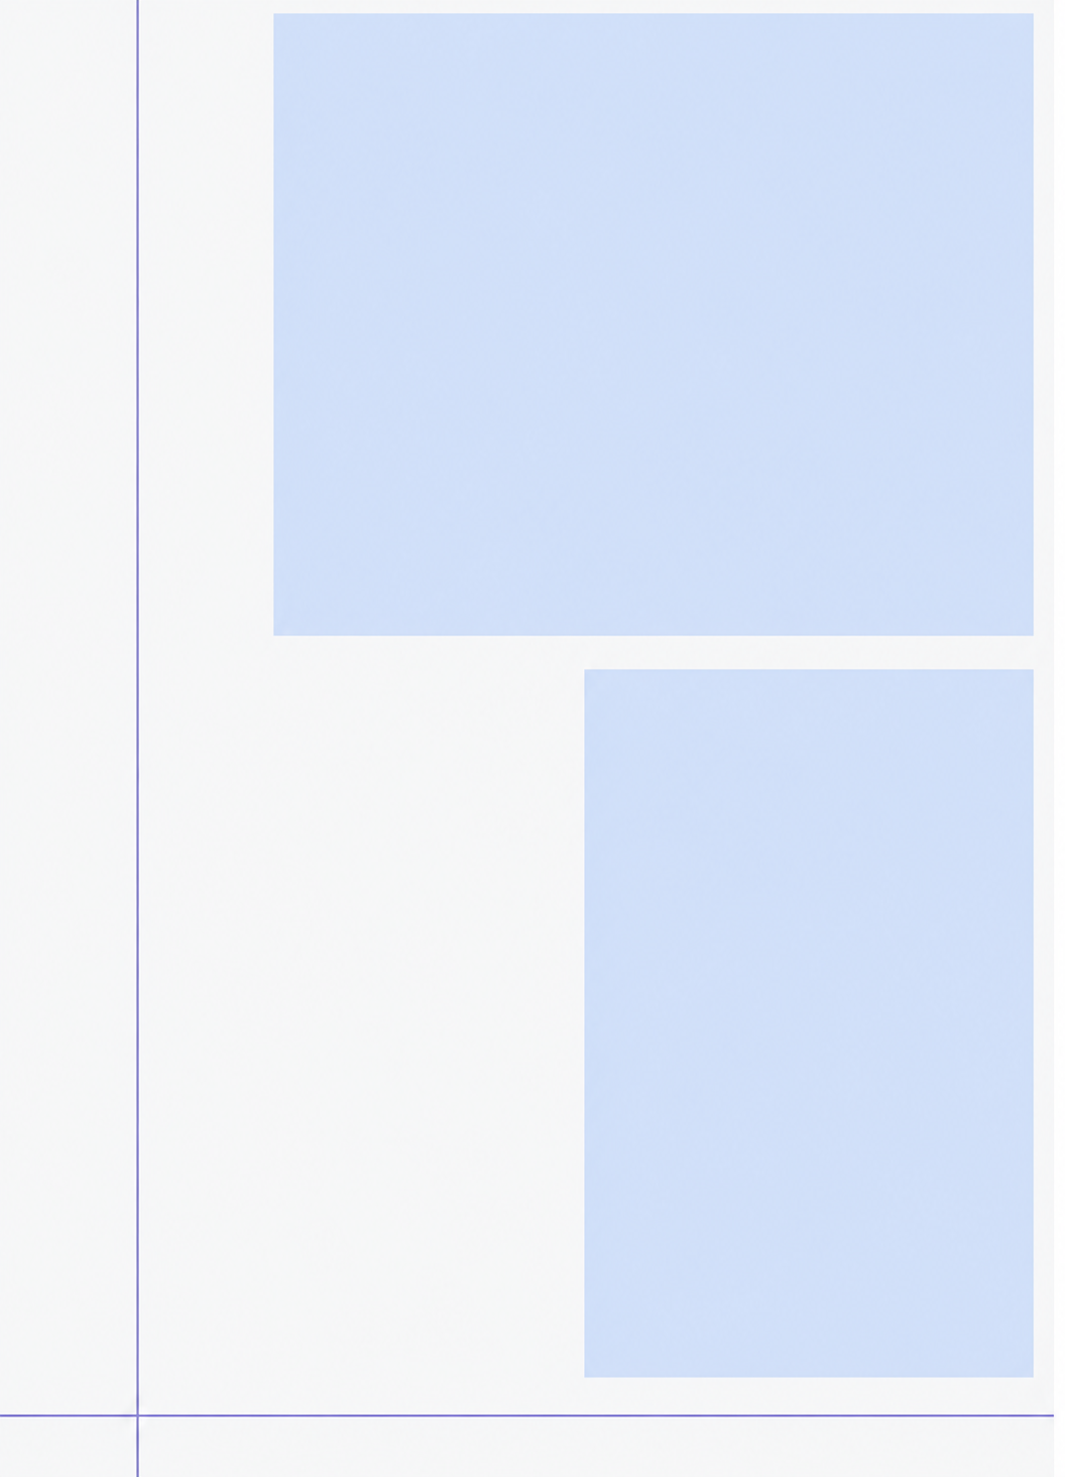
\includegraphics{GBU-symbol-top.png}%
      };
  \end{tikzpicture}%
}

\begin{center}
  \vspace*{5mm}
  %\gbulogo{72mm}\par
  \vspace{29mm}
  {\color{GBUBlueDark}\sffamily\coverxingkai\bfseries\fontsize{39}{39}\selectfont
   第三届大湾区拓扑会议\par}
  \vspace{25mm}
  {\color{GBUBlue}\sffamily\coverxingkai\bfseries\fontsize{35}{20}\selectfont
   会议手册\par}
  \vspace{20mm}
  {\color{GBUBlueDark}\sffamily\coverenglish\fontsize{25}{14}\selectfont
   Greater Bay Area Topology Conference 2026\par}\vspace{3mm}
  


  \vspace{55mm}
  \diamondrule
  %\vspace{5mm}
  {\color{GBUBlueDark}\sffamily\coverenglish\bfseries\fontsize{20}{25}\selectfont
   2026/11/21--23\par}
  \vspace{1mm}
  %{\color{GBUBlue}\sffamily\coverxingkai\fontsize{10}{13}\selectfont
  % 2026/11/21--23 \par}
  \vspace{5mm}
  {\color{GBUBlueDark}\sffamily\coverxingkai\bfseries \fontsize{20}{14} 主办单位：大湾区大学理学院\par}
\end{center}
\begin{tikzpicture}[remember picture,overlay]
  \node[
    anchor=south east,
    inner sep=0pt
  ] at ([xshift=-7mm,yshift=10mm]current page.south east) {
    \begin{minipage}{72mm}
      \centering
      \gbulogo{72mm}
    \end{minipage}
  };
\end{tikzpicture}
\clearpage
\restoregeometry

% Blank inside cover: no header, motto, page number, or other printed marks.
\thispagestyle{empty}
\thispdfpagelabel{空白页}
\null
\clearpage
\pagenumbering{arabic}
\hypersetup{pageanchor=true}
% --------------------------------------------------------------------------
% Conference information
% --------------------------------------------------------------------------
\section{会议概览}

大湾区拓扑会议旨在促进粤港澳大湾区及跨区域拓扑学及相关领域专家学者之间的交流，促进学者之间的深入讨论与合作。

\vspace{0.8em}
\renewcommand{\arraystretch}{1.45}
\arrayrulecolor{GBURule}
\noindent
\begin{tabularx}{\textwidth}{B{3.2cm}Y}
  \toprule
  会议名称 & 第三届大湾区拓扑会议\\
  英文名称 & Greater Bay Area Topology Conference 2026\\
  会议主题 & 流形拓扑与拓扑数据分析\\
  会议日期 & 2026年11月21日--23日\\
  报告时间 & 11月21--22日全天、11月23日上午\\
  主办单位 & 大湾区大学理学院\\
  会议地点 & 大湾区大学松山湖校区\\
  具体会场 & 教学楼 B206（21--22日），产研楼东塔 E502（23日） \\
  住宿酒店 & 湾大松山湖学术交流中心酒店\\
  用餐安排 & 食堂/酒店自助/盒饭（详见会议日程）\\
  会议网站 & \href{https://gbatc.github.io}{https://gbatc.github.io/}\\
  \bottomrule
\end{tabularx}

\vspace{1.2em}
\noindent
\begin{tikzpicture}
  \fill[GBUBlueLight,rounded corners=3pt] (0,0) rectangle (\textwidth,1.65);
  \fill[GBUOrange] (0,0) rectangle (0.12,1.65);
  \node[
    anchor=west,
    text width=\dimexpr\textwidth-1.0cm\relax,
    align=left
  ] at (0.55,0.82) {%
    \small\color{GBUText}
    11月21日共5场报告，22日共6场报告，23日共3场报告，每场50分钟。
    23日会场更换为产研楼东塔 E502，请留意。报告摘要按报告顺序排列。
  };
\end{tikzpicture}

\vspace{1.0em}
\subsection*{会议期间联系方式}
\small
\renewcommand{\arraystretch}{1.45}
\noindent
\begin{tabularx}{\textwidth}{B{2.6cm}Y L{3.6cm}}
  \toprule
  姓名 & \textbf{邮箱} & \textbf{手机}\\
  \midrule
  李鹏程 & \href{mailto:lipcaty@gbu.edu.cn}{lipcaty@gbu.edu.cn} & \mbox{13161005509}\\
  王靖文 & \href{mailto:wangjw@gbu.edu.cn}{wangjw@gbu.edu.cn} & \mbox{13060696196}\\
  \bottomrule
\end{tabularx}

\begin{center}
  \vspace{0.8em}
  
\includegraphics[width=28mm]{GBATC_website_QR.png}\par
  \vspace{0.3em}
  {\small 会议网页：扫码查看最新日程及会议信息}
\end{center}
\normalsize

\clearpage
\renewcommand{\contentsname}{目录}
\setcounter{tocdepth}{1}
{\hyphenpenalty=10000\exhyphenpenalty=10000\sloppy
\tableofcontents}

% --------------------------------------------------------------------------
% Schedule
% --------------------------------------------------------------------------
\clearpage
\section{会议日程 / \coverenglish Schedule}
\subsection{11月21日（星期六）}
\noindent\textcolor{GBUBlueDark}{\textbf{会场：教学楼 B206}}\par
\vspace{0.6em}
\begingroup
\small\centering
\renewcommand{\arraystretch}{1.65}\setlength{\tabcolsep}{5pt}
\renewcommand{\tabularxcolumn}[1]{m{#1}}
\noindent\begin{tabularx}{\textwidth}{|D{2.15cm}|S|D{1.25cm}|D{1.25cm}|}\hline
\rowcolor{GBUBlueLight}\textbf{时间}&\centering\arraybackslash\textbf{报告题目}&\textbf{报告人}&\textbf{主持人}\\\hline
08:30--08:40 & 开幕式 & --- & 李鹏程\\\hline
08:40--09:30 & The Kähler Degrees of Self-Maps of Generalized Grassmannians & 段海豹 & 高红铸\\\hline
\rowcolor{black!3}09:30--10:00 & \multicolumn{3}{c|}{合影与自由交流}\\\hline
10:00--10:50 & Reduced characteristic number criteria for equivariant bordisms & 吕志 & 高红铸\\\hline
\rowcolor{black!3}10:50--11:00 & \multicolumn{3}{c|}{休息}\\\hline
11:00--11:50 & Some questions related to free-by-cyclic groups and tubular groups & 叶圣奎 & 杨海波\\\hline
\rowcolor{black!3}12:00--14:00 & \multicolumn{3}{c|}{午餐（学校食堂）}\\\hline
14:30--15:20 & 基于计算拓扑的拓扑理解与拓扑控制 & 蔺宏伟 & 朱一飞\\\hline
\rowcolor{black!3}15:20--15:40 & \multicolumn{3}{c|}{自由交流}\\\hline
15:40--16:30 & Persistent Local Laplacian Prediction of Protein--Ligand Binding Affinities & 刘健 & 朱一飞\\\hline
\rowcolor{black!3}17:30起 & \multicolumn{3}{c|}{晚宴（顺德了然馆）}\\\hline
\end{tabularx}\par\endgroup

\clearpage\section*{会议日程 / \coverenglish Schedule}
\subsection{11月22日（星期日）}
\noindent\textcolor{GBUBlueDark}{\textbf{会场：教学楼 B206}}\par
\vspace{0.6em}
\begingroup
\small\centering
\renewcommand{\arraystretch}{1.65}\setlength{\tabcolsep}{5pt}
\renewcommand{\tabularxcolumn}[1]{m{#1}}
\noindent\begin{tabularx}{\textwidth}{|D{2.15cm}|S|D{1.25cm}|D{1.25cm}|}\hline
\rowcolor{GBUBlueLight}\textbf{时间}&\centering\arraybackslash\textbf{报告题目}&\textbf{报告人}&\textbf{主持人}\\\hline
09:00--09:50 & The existence of $SC^p$ metrics on manifolds which are like the octonionic projective plane & 苏阳 & 范飞飞\\\hline
\rowcolor{black!3}09:50--10:00 & \multicolumn{3}{c|}{休息}\\\hline
10:00--10:50 & 非正截面曲率黎曼度量模空间的拓扑 & 江怡 & 范飞飞\\\hline
\rowcolor{black!3}10:50--11:10 & \multicolumn{3}{c|}{自由交流}\\\hline
11:10--12:00 & Linear circle quotients of products of odd-dimensional spheres: classification and geometric applications & 沈文 & 曾昊智\\\hline
\rowcolor{black!3}12:00--14:00 & \multicolumn{3}{c|}{午餐（酒店自助餐）}\\\hline
14:00--14:50 & Topological obstructions to geometric positivity on Calabi-Yau manifolds & 李平 & 赵浩\\\hline
\rowcolor{black!3}14:50--15:00 & \multicolumn{3}{c|}{休息}\\\hline
15:00--15:50 & Rational ellipticity of Riemannian manifolds & 陈小杨 & 赵浩\\\hline
\rowcolor{black!3}15:50--16:10 & \multicolumn{3}{c|}{自由交流}\\\hline
16:10--17:00 & Whitney-Form-Based Cellular Sheaves: Construction, Laplacians, and Flat-Transport Moduli & 陈羽 & 杨会军\\\hline
\rowcolor{black!3}17:20起 & \multicolumn{3}{c|}{晚餐（盒饭）}\\\hline
\end{tabularx}\par\endgroup

\clearpage\section*{会议日程 / \coverenglish Schedule}
\subsection{11月23日（星期一）}
\noindent\textcolor{GBUBlueDark}{\textbf{会场：产研楼东塔 E502（会场变更！）}}\par
\vspace{0.6em}
\begingroup
\small\centering
\renewcommand{\arraystretch}{1.65}\setlength{\tabcolsep}{5pt}
\renewcommand{\tabularxcolumn}[1]{m{#1}}
\noindent\begin{tabularx}{\textwidth}{|D{2.15cm}|S|D{1.25cm}|D{1.25cm}|}\hline
\rowcolor{GBUBlueLight}\textbf{时间}&\centering\arraybackslash\textbf{报告题目}&\textbf{报告人}&\textbf{主持人}\\\hline
09:00--09:50 & Towards a topological trinity for speech intelligence & 朱一飞 & 杜晓明\\\hline
09:50--10:40 & 待定 / TBA & 颜延 & 杜晓明\\\hline
\rowcolor{black!3}10:40--11:00 & \multicolumn{3}{c|}{自由交流}\\\hline
11:00--11:50 & On the boundedness of almost flat $\mathrm{Spin}^c$ manifolds & 黄瑞芝 & 古星\\\hline
\rowcolor{black!3}12:00--14:00 & \multicolumn{3}{c|}{会议闭幕、午餐（盒饭）与自由讨论}\\\hline
\end{tabularx}\par\endgroup

\vspace{1.2em}
\subsection{会后学术报告 /\coverenglish Post-conference Talks}

\noindent
以下两场报告为独立安排的学术活动，
不属于本次会议正式议程，欢迎有兴趣的参会者参加。

\medskip
\noindent
\textcolor{GBUBlueDark}{%
  \textbf{时间：14:30--16:30 \qquad 会场：产研楼东塔 E502}%
}\par
\vspace{0.6em}

\begingroup
\small\centering
\renewcommand{\arraystretch}{1.65}
\setlength{\tabcolsep}{5pt}
\renewcommand{\tabularxcolumn}[1]{m{#1}}

\noindent
\begin{tabularx}{\textwidth}
  {|D{2.15cm}|S|D{1.25cm}|D{1.25cm}|}
\hline
\rowcolor{GBUBlueLight}
\textbf{时间} &
\textbf{报告题目} &
\textbf{报告人} &
\textbf{主持人}\\
\hline
14:30--15:20 & A counterexample to cohomological rigidity of toric manifolds & 龚涛 & 李鹏程\\
\hline
15:40--16:30 & Topological complexity of enumerative problems in algebraic geometry & 古星 & 李鹏程\\
\hline
\end{tabularx}
\par\endgroup

% --------------------------------------------------------------------------
% Abstracts: titles and abstracts are preserved from the submitted sources.
% --------------------------------------------------------------------------
\clearpage
\phantomsection
\addcontentsline{toc}{section}{报告信息 / \coverenglish Talk Information}
% White divider page avoids a full-page colour background in print.
\begin{center}
  \vspace*{50mm}
  \gbulogo{58mm}\par
  \vspace{30mm}
  {\color{GBUBlueDark}\sffamily\coverxingkai\bfseries\fontsize{38}{38}\selectfont
   报告信息\par}
  \vspace{2mm}
  {\color{GBUBlue}\sffamily\coverenglish\fontsize{25}{21}\selectfont
   Talk Information\par}
  \vspace{9mm}
  \vfill
  {\color{GBUBlueDark}\sffamily\coverxingkai 题目摘要按报告顺序排列\par}
\end{center}
\thispagestyle{printdivider}
\clearpage


\begin{talkabstract}{The Kähler Degrees of Self-Maps of Generalized Grassmannians}{段海豹}{中科院数学所}{11月21日 08:40--09:30}
Generalized Grassmannians constitute a fundamental class of flag manifolds associated with Lie groups. This talk addresses the classification of their self-maps in terms of the induced endomorphisms of their cohomology rings. Our main result reveals a striking rigidity phenomenon: despite the rich and intricate structure of these cohomology rings, the induced endomorphisms fall into only two natural types---Adams operations determined by the Kähler degree and Dynkin symmetries induced by automorphisms of the Dynkin diagram.
\vspace{1mm}\bio{段海豹，中国科学院数学与系统科学研究院研究员，主要从事代数拓扑、微分拓扑与代数几何研究。1987年获北京大学博士学位，在舒伯特演算、齐性空间的上同调及流形映射等方面取得系列成果。曾获国家自然科学二等奖、国家教委科技进步二等奖、人事部优秀博士后奖、国家教委优秀跨世纪人才、中国数学会陈省身数学奖等。} 
\end{talkabstract}


\begin{talkabstract}{Reduced characteristic number criteria for equivariant bordisms}{吕志}{复旦大学}{11月21日 10:00--10:50}
Classical equivariant bordism theories require computing the full collection of equivariant characteristic numbers to detect whether an equivariant manifold bounds equivariantly or not. In this talk, we consider simplified equivariant bordism characterizations for two families of equivariant manifolds with isolated fixed points: unitary $T^k$-manifolds and closed smooth $(\mathbb{Z}_2)^k$-manifolds. For a unitary $T^k$-manifold $M$ with isolated fixed points, we establish an equivariant unitary bordism criterion built entirely from a single polynomial of equivariant Chern classes. We further introduce the minimal distinguishing degree and obtain two key inequalities that capture the interplay between $\dim(M)$ and the Euler characteristic $\chi(M)$ through this minimal distinguishing degree. This is also applied to Kosniowski's conjecture and its toric generalization. By contrast, for a closed smooth $(\mathbb{Z}_2)^k$-manifold with isolated fixed points, we derive a more concise equivariant bordism criterion relying solely on the powers of the top equivariant Stiefel--Whitney class. Our new criteria substantially reduce computational demands. This is joint work with Runze Chen and Leqi Yang.
\vspace{1mm}\bio{吕志，男，复旦大学 数学科学学院教授，博士生导师。主要从事代数拓扑、变换群以及环面拓扑研究，在等变协边分类及不变量、广义Smith猜想、Kosniowski猜想的研究上取得重要研究成果，发表在\emph{Math. Ann., Trans AMS, IMRN, Math. Z., AGT，Math. Res. Lett.}等期刊上。多次主持国家自然科学基金及教育部博士学科点基金项目等。曾获教育部自然科学奖二等奖（独立）。}
\end{talkabstract}


\begin{talkabstract}{Some questions related to free-by-cyclic groups and tubular groups}{叶圣奎}{上海纽约大学}{11月21日 11:00--11:50}
We prove that a CAT(0) free-by-cyclic tubular group with one vertex is virtually special, but many of them cannot virtually act freely and cocompactly on CAT(0) cube complexes. This partially confirms a question of Brady--Soroko and answers a question of Lyman in the negative. Furthermore, we provide examples of free-by-cyclic groups amalgamated along cyclic subgroups that are not virtually free-by-cyclic. This answers negatively a question of Hagen--Wise. Lastly, we exhibit an example of a cyclic-subgroup-separable tubular group that does not have the property (VRC) (i.e. every cyclic subgroup is a virtual retract). This answers a question of Minasyan in the negative. This is a joint work with Xiaolei Wu.
\vspace{1mm}\bio{叶圣奎，上海纽约大学数学实践教授。2012年获新加坡国立大学数学博士学位，曾任牛津大学数学研究所西蒙斯博士后研究员及西交利物浦大学讲师、高级讲师。主要从事拓扑学与几何群论研究，特别关注流形及非正曲率空间上的群作用，以及群的代数性质与几何拓扑性质之间的联系。}
\end{talkabstract}


\begin{talkabstract}{\coverxingkai 基于计算拓扑的拓扑理解与拓扑控制}{蔺宏伟}{浙江大学}{11月21日 14:30--15:20}
计算机辅助几何设计（CAGD）的主要目标是对三维几何模型进行设计与处理，其中拓扑结构与几何形状是两个关键组成部分。然而，传统CAGD 侧重于几何外形设计与处理，缺乏用于理解和控制三维模型拓扑结构的系统方法论。随着建模技术应用范围的扩大，模型设计与处理中涉及拓扑理解和控制的挑战日益突出，这在微结构和分子结构设计等领域尤为明显。因此，迫切需要开发系统且有效的拓扑理解与控制理论及技术。本报告介绍了以持续同调（persistent homology）为核心工具的计算拓扑（computational topology），如何系统解决三维几何模型在拓扑理解与拓扑控制方面的关键挑战，进而发展计算机辅助拓扑设计（Computer Aided Topological Design）系统理论和方法。
\vspace{1mm}\bio{蔺宏伟，浙江大学数学科学学院教授、博士生导师。1996年获浙江大学学士学位，2004年获浙江大学博士学位。主要从事计算机辅助几何设计、计算机辅助拓扑设计、拓扑数据分析及量子图形学研究，发展了渐进迭代逼近方法及基于持续同调的拓扑设计方法。曾获国家自然科学奖二等奖、陆增镛CAD \& CG高科技奖一等奖等。}
\end{talkabstract}

\begin{talkabstract}{Persistent Local Laplacian Prediction of Protein--Ligand Binding Affinities}{刘健}{重庆理工大学}{11月21日 15:40--16:30}
Accurate prediction of protein--ligand binding affinity remains a central challenge in structure-based drug discovery. The effectiveness of machine learning models critically depends on the quality of molecular representations, for which advanced mathematical frameworks provide powerful tools. In this work, we employ a novel mathematical theory, termed the persistent local Laplacian (PLL), to construct molecular descriptors that capture localized geometric and topological features of biomolecular structures. The PLL framework addresses key limitations of traditional topological data analysis methods, such as persistent homology and the persistent Laplacian, which are often insensitive to local structural variations, while maintaining high computational efficiency. The resulting molecular descriptors are integrated with advanced machine learning algorithms to develop accurate predictive models for protein--ligand binding affinity. The proposed models are systematically evaluated on three well-established benchmark datasets, including PDBbind-v2007, PDBbind-v2013, and PDBbind-v2016, demonstrating consistently strong and competitive predictive performance. Computational results show that the PLL-based models outperform existing approaches, highlighting their potential as a powerful tool for drug discovery, protein engineering, and broader applications in science and engineering.
\vspace{1mm}\bio{刘健，重庆理工大学助理教授，硕士生导师。主要从事代数拓扑领域的研究，研究兴趣包括有理同伦论、模型范畴和拓扑数据分析。在\emph{Nature Machine Intelligence, Homology, Homotopy and Applications}等期刊发表论文十余篇，主持国家自然科学基金青年项目。}
\end{talkabstract}

\clearpage 

\begin{talkabstract}{The existence of $\mathrm{SC}^p$ metrics on manifolds which are like the octonionic projective plane}{苏阳}{中科院数学所}{11月22日 09:00--09:50}
A Riemannian metric has the $\mathrm{SC}^p$ property at a point $p$ if every geodesic issued from $p$ is simply closed and all these geodesics have the same prime length. We show that smooth closed simply connected manifolds whose homology groups are isomorphic to that of the octonionic projective plane admit such metrics. This is a joint work with Martin Kerin and Chao Qian.
\vspace{1mm}\bio{苏阳，中国科学院数学与系统科学研究院研究员、博士生导师。2007年获德国海德堡大学数学博士学位，同年进入中国科学院数学研究所工作。主要从事高维流形拓扑研究，研究方向包括流形分类、群作用、映射类群及几何结构。研究成果发表于 \emph{Duke Mathematical Journal、Geometry \& Topology、Mathematische Annalen} 等期刊。}
\end{talkabstract}


\begin{talkabstract}{\coverxingkai 非正截面曲率黎曼度量模空间的拓扑}{江怡}{首都师范大学}{11月22日 10:00--10:50}
设$M$为一光滑闭流形，其上存在非正截面曲率的黎曼度量。$M$上所有非正截面曲率黎曼度量构成的空间，在$M$的自微分同胚群拉回作用下的商空间，称为$M$的非正截面曲率度量模空间。本报告将介绍F.T. Farrell与报告人在该模空间拓扑方面的近期合作研究进展。
\vspace{1mm}\bio{江怡，首都师范大学交叉科学研究院研究员。2014年获中国科学院大学博士学位，曾在清华大学丘成桐数学科学中心从事博士后研究并任助理教授。主要研究代数拓扑与几何拓扑，特别是高维流形拓扑、流形上的群作用，以及曲率受限黎曼度量空间的拓扑。}
\end{talkabstract}


\begin{talkabstract}{Linear circle quotients of products of odd-dimensional spheres: classification and geometric applications}{沈文}{温州大学}{11月22日 11:10--12:00}
In this talk, we study the topology and geometry of orbit manifolds arising from free diagonal linear circle actions on $S^{2n+1}\times S^{2n+1}$. We first present an explicit arithmetic classification of these manifolds up to PL homeomorphism for every $n\geq 1$. We then discuss more refined homotopy and diffeomorphism classification results in dimensions $9$ and $13$. Finally, we explain two geometric applications of the diffeomorphism classification. This is joint work with Su Yang.
\vspace{1mm}\bio{沈文，温州大学数理学院讲师。2018年获南开大学硕士学位，2022年获首都师范大学博士学位，师从方复全院士。2023年至2025年在首都师范大学从事博士后研究，2025年加入温州大学。主要研究代数拓扑、高维流形拓扑与同伦论。}
\end{talkabstract}


\begin{talkabstract}{Topological obstructions to geometric positivity on Calabi-Yau manifolds}{李平}{复旦大学}{11月22日 14:00--14:50}
一般认为卡-丘流形的拓扑型具有较强的刚性，即不能承载某些正性或负性几何结构。在这个报告中我将回顾一些相关背景并在某些情形给出一些不存在结果来支撑这个刚性猜测。
\vspace{1mm}\bio{李平，复旦大学数学科学学院教授、博士生导师，国家优秀青年科学基金获得者。2004年获武汉大学学士学位，2009年获北京大学博士学位，曾在同济大学工作，2023年加入复旦大学。主要从事流形拓扑、微分几何及相关交叉领域研究，关注流形与向量丛的几何结构、示性数及其拓扑约束。}
\end{talkabstract}


\begin{talkabstract}{Rational ellipticity of Riemannian manifolds}{陈小杨}{同济大学}{11月22日 15:00--15:50}
A compact simply connected Riemannian manifold is rationally elliptic, if it has finite dimensional rational homotopy groups. We will discuss some recent results on rational ellipticity of Riemannian manifolds.
\vspace{1mm}\bio{陈小杨，同济大学数学科学学院长聘副教授。主要从事黎曼几何及相关拓扑问题研究，研究兴趣包括非负截面曲率流形的几何与拓扑、群作用，以及人工智能辅助数学研究。在 \emph{Geometry \& Topology}、\emph{Advances in Mathematics}、\emph{Mathematische Annalen} 等期刊发表多篇论文，曾主持国家自然科学基金青年及面上项目。}
\end{talkabstract}

\begin{talkabstract}{Whitney-Form-Based Cellular Sheaves: Construction, Laplacians, and Flat-Transport Moduli}{陈羽}{新加坡国立大学}{11月22日 16:10--17:00}
In graph neural networks, message passing primarily characterizes relationships through vertices and edges. High-dimensional data, however, necessitates comparisons between higher-dimensional simplices. Simplicial complex models and sheaf models provide mechanisms for high-dimensional message passing. Consequently, constructing cellular sheaves with favorable geometric and topological properties on simplicial complexes is of significant importance for research into topological deep learning. In this talk, we introduce the Whitney-Form-Based Cellular Sheaves. By reconstructing moments, we derive oriented stalk metrics and combine them with flat transport defined over the partially ordered set of faces of a simplicial complex, and yielding the corresponding sheaf Laplacian. We will discuss the fundamental properties of these cellular sheaves, the tools they offer for investigating the geometry and topology of spaces, and their potential applications in topological deep learning.
\vspace{1mm}\bio{陈羽，新加坡国立大学在读博士研究生（本硕浙江大学），导师韩飞。他的研究方向包括拓扑数据分析、几何深度学习和拓扑深度学习等，目前已在Neural Networks, Computer-Aided Design等多个国际著名期刊上发表了学术论文。}
\end{talkabstract}

\clearpage 







\begin{talkabstract}{Towards a topological trinity for speech intelligence}{朱一飞}{南方科技大学}{11月23日 09:00--09:50}
Over more than a decade of interdisciplinary research in topological analysis and deep learning with image and video data, Carlsson and colleagues have established a paradigm for detecting and utilizing their topological distributions and dynamics that incorporate the three interacting areas of data science (of signals), artificial intelligence (of machines), and neuroscience (of humans).  In this talk, I’ll report on progress towards topologically understanding speech data both by analogy and in contrast.  Specifically, we integrate topological time series analysis with machine learning to capture structural features in consonant classification, while enhancing interpretability and robustness against noise compared to traditional techniques.  This is joint work with Zeyang Ding, Pingyao Feng, Qingrui Qu, Siheng Yi, Zhiwang Yu, and Haiyu Zhang.
\vspace{1mm}\bio{朱一飞，南方科技大学数学系助理教授。2007年获北京大学学士学位，2013年获美国明尼苏达大学数学博士学位，曾任美国西北大学访问助理教授。主要研究代数拓扑及其与代数几何、数论的相互作用，同时探索拓扑与几何方法在凝聚态物理、时间序列分析和人机交互等领域的应用。}
\end{talkabstract}


\begin{talkabstract}{拓扑数据分析的生物医学信号应用实践}{颜延}{中科院深圳先进技术研究院}{11月23日 09:50--10:40}
生物医学信号常受噪声与伪迹干扰，传统方法稳定性有限。拓扑数据分析（TDA）通过持续同调刻画信号的多尺度结构，为生物医学信号提供鲁棒表征。本报告围绕“信号—点云—拓扑特征”的实践流程，介绍如何将时间序列转化为拓扑特征，并结合生物医学工程领域典型案例进行介绍。最后讨论参数选择、计算效率与可解释性等落地问题，为TDA在生物医学信号领域的应用实践提供参考。
\vspace{1mm}\bio{颜延，中国科学院深圳先进技术研究院高级工程师。2012年于哈尔滨工业大学完成仪器科学与技术本硕阶段学习，2020年获中国科学院大学计算机应用技术博士学位。主要从事计算拓扑在机器学习与生物医学信号处理中的应用研究，关注拓扑数据分析、拓扑几何深度学习及生物医学智能分析模型的设计。}
\end{talkabstract}



\begin{talkabstract}{On the boundedness of almost flat $\mathrm{spin}^c$ manifolds}{黄瑞芝}{中科院数学所}{11月23日 11:00--11:50}
The Farrell-Zdravkovska-Yau conjecture asserts that every almost flat manifold bounds a compact manifold. We prove this conjecture for spin$^c$ almost flat manifolds in low dimensions, or in arbitrary dimensions with suitable holonomy groups.

In contrast to the group-theoretic techniques employed in earlier works, we introduce a new topological approach to tackle this conjecture. Our method combines the Atiyah-Singer index theorem for spin$^c$ manifolds with the Hopkins-Singer-type integral lifts of Wu classes in algebraic topology.

This is a joint work with Fei Han and Weiping Zhang.
\vspace{1mm}\bio{黄瑞芝，中国科学院数学与系统科学研究院副研究员、博士生导师。2017年获新加坡国立大学数学博士学位，此后在中国科学院数学与系统科学研究院从事博士后及科研工作。主要研究代数拓扑及其在流形拓扑、微分几何和数学物理中的应用，关注非稳定同伦论、流形与规范群的同伦性质，以及指标理论中的拓扑问题。}
\end{talkabstract}

\clearpage 

\begin{talkabstract}{A counterexample to cohomological rigidity of toric manifolds}{龚涛}{西安大略大学（加拿大）}{11月23日 14:30--15:20}
The long-standing cohomological rigidity problem for toric manifolds asks whether the integral cohomology ring of a toric manifold determines its diffeomorphism type, homeomorphism type, or homotopy type. We construct two toric manifolds of complex dimension four whose integral cohomology rings are isomorphic but which are not homotopy equivalent, thereby giving a negative answer to this problem. This is joint work with Yingxin Li.

\vspace{1mm}
\bio{龚涛，西安大略大学数学博士，师从 Matthias Franz 教授，本科及硕士毕业于北京师范大学。主要研究方向为代数拓扑、同伦论与环面拓扑，重点研究环面簇的拓扑结构、反射群作用、上同调不变量及上同调刚性问题。
近年来围绕环面簇的同伦型与上同调环结构开展了一系列研究，相关成果发表于HHA等数学期刊。近期与合作者构造了两个整数上同调环同构但不同伦等价的复四维光滑环面簇，给出了 Masuda–Suh 于 2007 年提出的上同调刚性猜想的一般性反例。曾在普林斯顿大学、加拿大数学会、菲尔兹数学科学研究所等学术机构及会议上作学术报告。}
\end{talkabstract}


\begin{talkabstract}{Topological complexity of enumerative problems in algebraic geometry}{古星}{西湖大学}{11月23日 15:40--16:30}
Typical enumerative problems in algebraic geometry include finding the $d$ roots of a generic polynomial in one variable of degree $d$, finding the $27$ lines on a smooth cubic surface, and their higher dimensional analogs. We introduce the concept of topological complexity of enumerative problems, which is a positive integer that measures the least possible number of “branches” in the algorithms that solves an 
enumerative problem up to an $\epsilon$ error. We are interested in the lower bounds of the topological complexity of enumerative problems. We introduce finite covering spaces associated to the enumerative problems and the concept of Schwarz genus of a covering space, 
which produces lower bounds of the topological complexity, and can be detected by cohomology. Finally, we present lower bounds of three enumerative problems.  
This is a joint work with Weiyan Chen.

\vspace{1mm}\bio{古星，2017年毕业于美
国伊利诺伊大学芝加哥分校，获博士学位。2017年11月-2020年1月于澳大利亚墨尔本
大学担任博士后，2020年2月-2021年1月在德国马克斯普朗克数学研究所从事博士后研
究工作，于 2022年4月全职加入西湖大学，担任理学院、理论科学研究院特聘研究员。
主要研究兴趣是同伦论以及李群和代数群的示性类理论。}
\end{talkabstract}

% --------------------------------------------------------------------------
% Transport information: concise, text-only, no map image.
% --------------------------------------------------------------------------
\clearpage
\section{交通与会场指引 / \coverenglish  Transportation and Venues}

\noindent\textbf{\color{GBUBlueDark}校区地址：}
大湾区大学松山湖校区（广东省东莞市松山湖大学路16号）。

\noindent\textbf{\color{GBUBlueDark}住宿酒店：}
\href{https://surl.amap.com/171OaF013g7T}{湾大松山湖学术交流中心酒店}。

\subsection*{会场安排}
\renewcommand{\arraystretch}{1.5}
\noindent\begin{tabularx}{\textwidth}{B{3.5cm}Y}
\toprule
11月21--22日 & 教学楼 B206\\
11月23日 & \textbf{产研楼东塔 E502（会场变更）}\\
\bottomrule
\end{tabularx}

\IfFileExists{GBU-campus-guide.jpg}{%
  \subsection*{校园导览}
  \noindent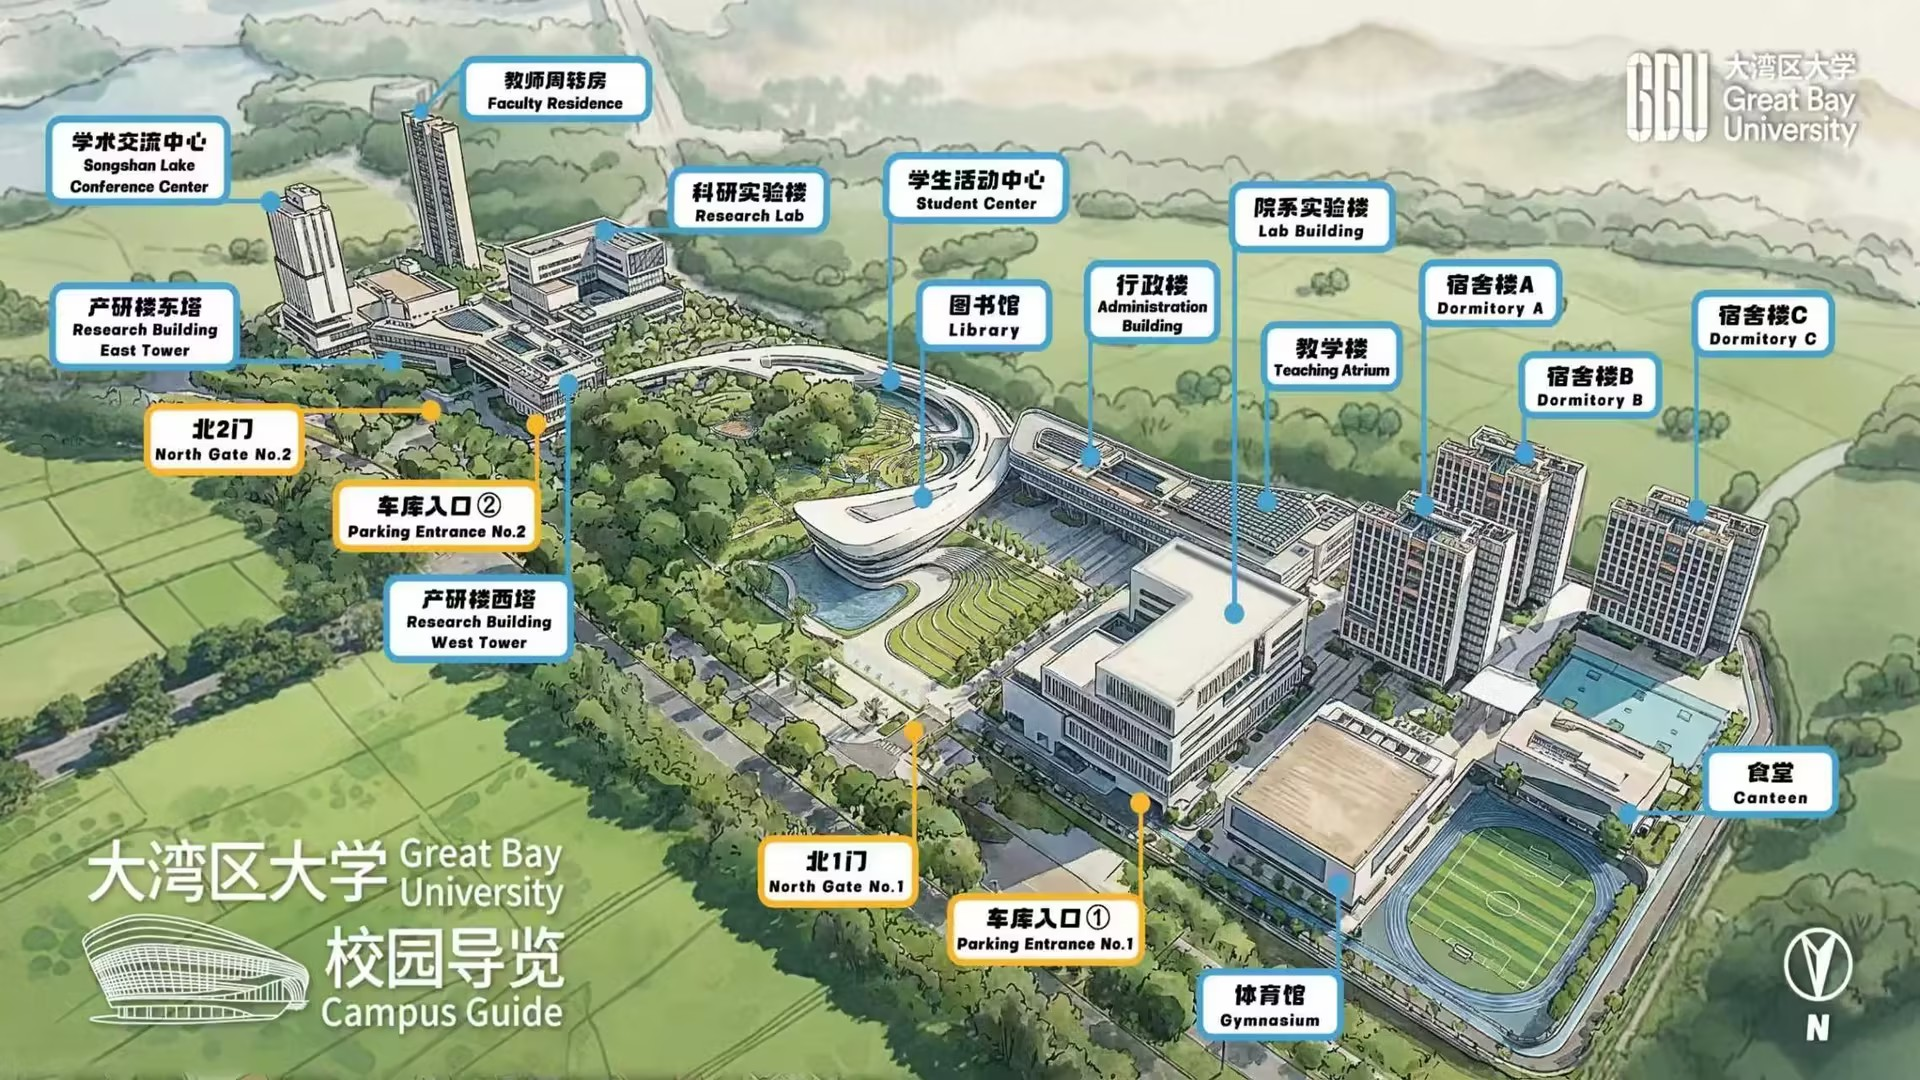
\includegraphics[width=\textwidth,height=11cm,keepaspectratio]{GBU-campus-guide.jpg}
  \par\small 本图用于校园建筑定位；具体教室及通行路线以现场导视为准。\normalsize
}{}


\subsection*{会务咨询}
李鹏程：13161005509；王靖文：13060696196。


\clearpage
\section{组织委员会 /\coverenglish  Organizers}
\renewcommand{\arraystretch}{1.5}
\noindent\begin{tabularx}{\textwidth}{B{5.7cm}Y}
\toprule
姓名 & \textbf{单位}\\\midrule
杜晓明 / Xiaoming Du & 华南理工大学\\
范飞飞 / Feifei Fan & 华南师范大学\\
李鹏程 / Pengcheng Li & 大湾区大学\\
梁灏 / Hao Liang&佛山大学\\
刘登品 / Dengpin Liu&桂林航天工业学院\\
邬恩信 / Enxin Wu & 汕头大学\\
谢恒 / Heng Xie & 中山大学\\
徐勐戬 / Mengjian Xu & 广西师范大学\\
徐鹏程 / Pengcheng Xu & 广东金融学院\\
赵浩 / Hao Zhao & 华南师范大学\\
朱一飞 / Yifei Zhu & 南方科技大学\\
\bottomrule
\end{tabularx}

\vspace{1em}\noindent\textbf{会务助理：}王靖文 / Jingwen Wang（大湾区大学）。

\clearpage
\section{参会人员 / \coverenglish Participants}
\noindent\small 按提供的参会名单顺序排列。\par
\renewcommand{\arraystretch}{1.28}
\small
\begin{longtable}{@{}C{0.9cm}L{5.0cm}L{8.8cm}@{}}
\toprule
\textbf{序号} & \textbf{姓名} & \textbf{单位}\\\midrule
\endfirsthead
\toprule
\textbf{序号} & \textbf{姓名} & \textbf{单位}\\\midrule
\endhead
\midrule\multicolumn{3}{r}{续下页}\\\endfoot
\bottomrule\endlastfoot
1 & Ali Danish & Dalian University of Technology\\
2 & 安妮 / Ni An & Southern University of Science and Technology\\
3 & 白琪峰 / Qifeng Bai & Changchun University of Technology\\
4 & 包汉桢 / Hanzhen Bao & Shanghai University of Finance and Economics\\
5 & 毕婉莹 / Wanying Bi & Chongqing University of Technology\\
6 & 陈小杨 / Xiaoyang Chen & Tongji University\\
7 & 陈羽 / Yu Chen & National University of Singapore\\
8 & 邓栋元 / Dongyuan Deng & Southern University of Science and Technology\\
9 & 杜晓明 / Xiaoming Du & South China University of Technology\\
10 & 段海豹 / Haibao Duan & AMSS, CAS\\
11 & 范飞飞 / Feifei Fan & South China Normal University\\
12 & 高红铸 / Hongzhu Gao & Beijing Normal University\\
13 & 高靖雯 / Jingwen Gao & Chongqing University of Technology\\
14 & 龚涛 / Tao Gong & University of Western Ontario\\
15 & 古星 / Xing Gu & Westlake University\\
16 & 何遵武 / Zunwu He & South China University of Technology\\
17 & 侯岐林 / Qilin Hou & Southern University of Science and Technology\\
18 & 黄瑞芝 / Ruizhi Huang & AMSS, CAS\\
19 & 江怡 / Yi Jiang & Capital Normal University\\
20 & 李平 / Ping Li & Fudan University\\
21 & 李鹏程 / Pengcheng Li & Great Bay University\\
22 & 李炫良 / Xuanliang Li & Guangdong University of Finance\\
23 & 李迎新 / Yingxin Li & Nankai University\\
24 & 林奕武 / Yiwu Lin & Guangdong University of Finance\\
25 & 蔺宏伟 / Hongwei Lin & Zhejiang University\\
26 & 刘健 / Jian Liu & Chongqing University of Technology\\
27 & 刘文琰 / Wenyan Liu & South China Agricultural University\\
28 & 吕志 / Zhi Lü & Fudan University\\
29 & Dana Melnikova & Tsinghua University\\
30 & 明杨 / Yang Ming & Hubei Polytechnic University\\
31 & 沈文 / Wen Shen & Wenzhou University\\
32 & 苏阳 / Yang Su & AMSS, CAS\\
33 & 田家承 / Jiacheng Tian & Zunyi Medical University\\
34 & 童浥尘 / Yichen Tong & Westlake University\\
35 & 王炜飚 / Weibiao Wang & Central South University\\
36 & 王云杰 / Yunjie Wang & Southern University of Science and Technology\\
37 & 文子杰 / Zijie Wen & Southern University of Science and Technology\\
38 & 邬恩信 / Enxin Wu & Shantou University\\
39 & 伍轩 / Xuan Wu & Southern University of Science and Technology\\
40 & 吴忠涛 / Zhongtao Wu & The Chinese University of Hong Kong\\
41 & 谢传龙 / Chuanlong Xie & Sun Yat-sen University\\
42 & 谢恒 / Heng Xie & Sun Yat-sen University\\
43 & 徐彬斌 / Binbin Xu & Hebei Normal University\\
44 & 徐鹏程 / Pengcheng Xu & Guangdong University of Finance\\
45 & 许远 / Yuan Xu & Xi'an Jiaotong University\\
46 & 颜延 / Yan Yan & Shenzhen Institute of Advanced Technology, CAS\\
47 & 杨海波 / Haibo Yang & Nanchang Hangkong University\\
48 & 杨会军 / Huijun Yang & Henan University\\
49 & 杨文慧 / Wenhui Yang & Southern University of Science and Technology\\
50 & 杨铮 / Zheng Yang & Sichuan University Auckland College\\
51 & 杨正霖 / Zhenglin Yang & Southern University of Science and Technology\\
52 & 叶圣奎 / Shengkui Ye & NYU Shanghai\\
53 & 曾昊智 / Haozhi Zeng & Huazhong University of Science and Technology\\
54 & 张前 / Qian Zhang & Westlake University\\
55 & 张枝磊 / Zhilei Zhang & Xi'an Shiyou University\\
56 & 赵浩 / Hao Zhao & South China Normal University\\
57 & 朱一飞 / Yifei Zhu & Southern University of Science and Technology\\
\end{longtable}\normalsize

% Back cover: full-sheet positioning, original aspect ratio, no cropping.
\clearpage
\hypersetup{pageanchor=false}
\thispagestyle{empty}
\thispdfpagelabel{封底}
\definecolor{BackCoverBackground}{RGB}{246,247,247}
\pagecolor{BackCoverBackground}
\begin{tikzpicture}[remember picture,overlay]
  \node[anchor=center,inner sep=0pt,outer sep=0pt]
    at (current page.center) {%
      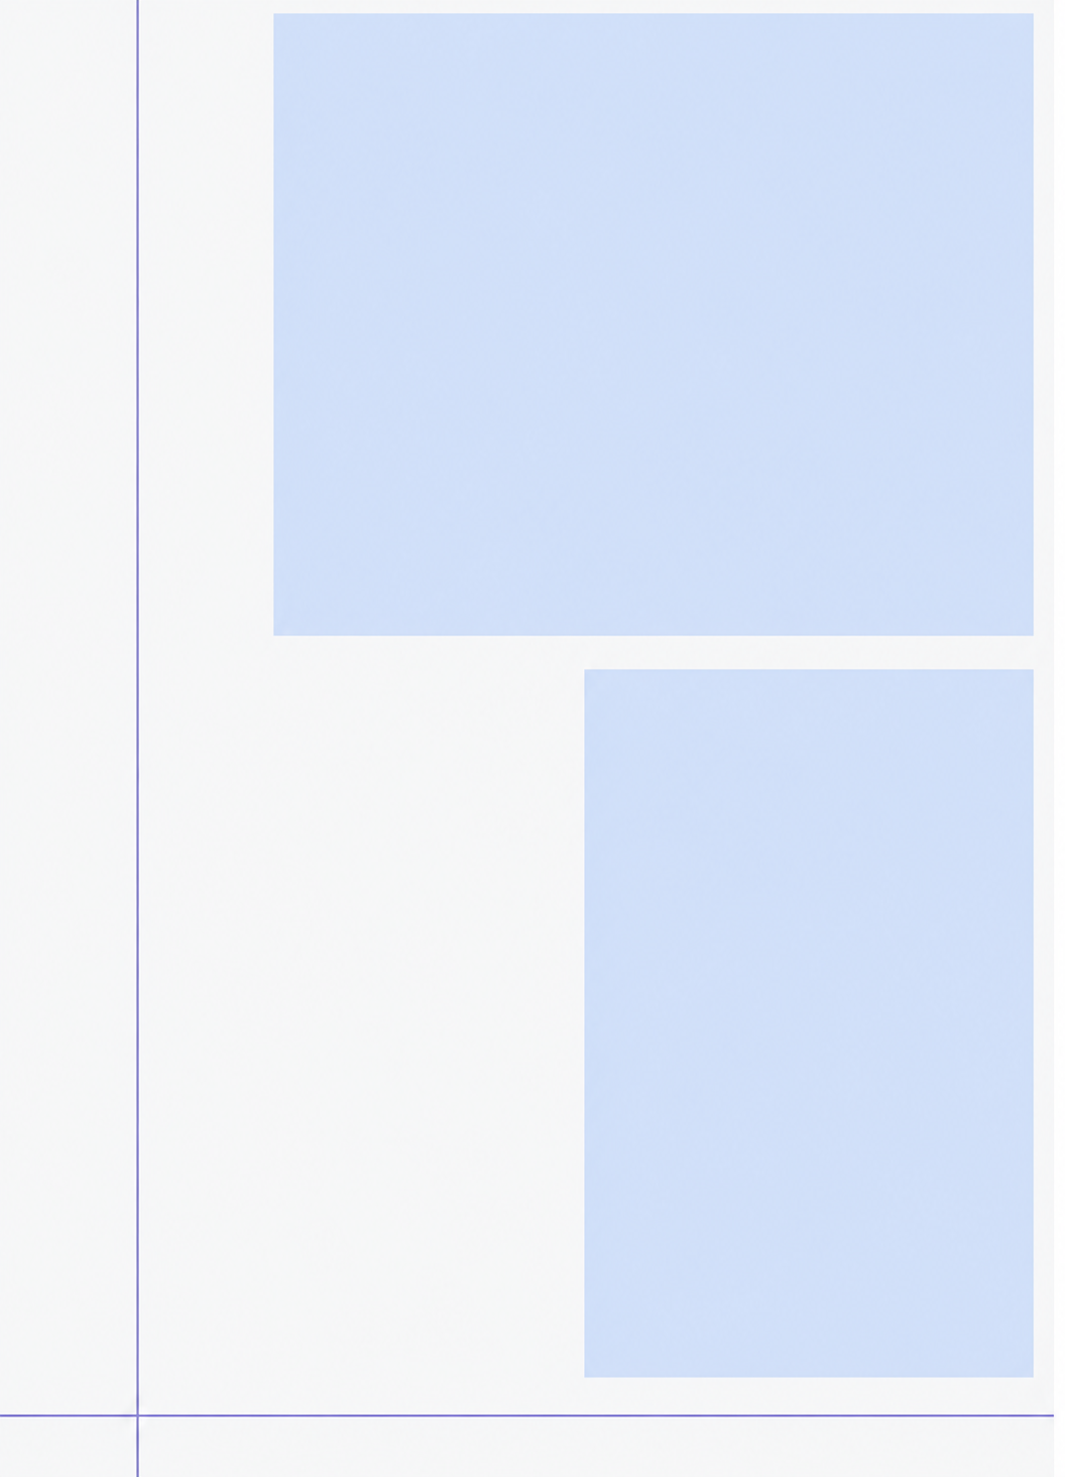
\includegraphics{GBU-symbol-top.png}%
    };
\end{tikzpicture}%

\begin{center}
  \vspace*{80mm}
  \gbulogo{90mm}
\end{center}  
\null
\clearpage
\nopagecolor
\end{document}
